% Two-page cheating paper LaTeX template
% Compile with XeLaTeX.
% Target: A4 landscape, four columns, exactly two rendered pages.
% After compiling, run:
%   python3 scripts/check_pdf_pages.py output.pdf --expect 2

\documentclass[UTF8,a4paper,landscape,fontset=none]{ctexart}

\usepackage[left=0.3cm,right=0.3cm,top=0.3cm,bottom=0.3cm]{geometry}
\usepackage{amsmath,amssymb,mathtools}
\usepackage{multicol}
\usepackage{xcolor}
\usepackage{graphicx}
\usepackage{tikz}
\usepackage{enumitem}
\usepackage{microtype}
\usetikzlibrary{arrows.meta,calc,positioning}

% macOS CJK fonts. Replace these if compiling on another system.
\setCJKmainfont{Songti SC}
\setCJKsansfont{Heiti SC}

\pagestyle{empty}
\setlength{\parindent}{0pt}
\setlength{\parskip}{0pt}
\setlength{\columnsep}{0.05cm}
\setlength{\columnseprule}{0pt}
\setlength{\emergencystretch}{1.5em}
\setlist{nosep,leftmargin=*,topsep=0pt,partopsep=0pt,parsep=0pt,itemsep=0pt}

\definecolor{keyblue}{HTML}{1476D4}
\definecolor{lightbox}{HTML}{F5F8FF}
\definecolor{warnred}{HTML}{C62828}

% Main size. If text looks too flat, use 6.5/7.0 or 6.5/7.1.
\newcommand{\tight}{\fontsize{6.5pt}{6.75pt}\selectfont}
\newcommand{\smalltight}{\fontsize{5.7pt}{5.9pt}\selectfont}
\newcommand{\tinytight}{\fontsize{4.9pt}{5.0pt}\selectfont}

% Section labels.
\newcommand{\chap}[1]{\par\textcolor{keyblue}{\sffamily\bfseries #1}\par}
\newcommand{\topic}[1]{\par\textcolor{keyblue}{\sffamily\bfseries #1}\par}
\newcommand{\warn}[1]{\textcolor{warnred}{\sffamily\bfseries #1}}
\newcommand{\kw}[1]{\textcolor{keyblue}{\sffamily\bfseries #1}}

% Compact formula / fact blocks.
\newcommand{\fact}[2]{\par\textcolor{keyblue}{\sffamily\bfseries #1}\quad #2\par}
\newcommand{\eqn}[1]{\par\(\displaystyle #1\)\par}
\newcommand{\twoline}[2]{\par\(\displaystyle #1\)\par[-1pt]\(\displaystyle #2\)\par}

% Figure helper. Put images under latex_build/image/ or image/.
\graphicspath{{./}{image/}{latex_build/image/}}
\newcommand{\pptfig}[2][0.72]{%
  \par\vspace{0.35pt}\noindent
  \makebox[\linewidth][c]{\includegraphics[width=#1\linewidth]{#2}}%
  \par\vspace{0.35pt}%
}

% Side-by-side card for tiny diagrams plus analysis.
\newcommand{\chanfont}{\fontsize{4.75pt}{4.85pt}\selectfont}
\tikzset{
  charr/.style={-{Latex[length=1.7mm]}, line width=0.28pt},
  chnode/.style={inner sep=0.3pt}
}
\newcommand{\chcard}[3]{%
  \par\vspace{0.45pt}\noindent
  \begin{minipage}[t]{0.43\linewidth}
    \vspace{0pt}
    \centering #2\par
  \end{minipage}\hfill
  \begin{minipage}[t]{0.54\linewidth}
    \vspace{0pt}
    {\chanfont\sffamily\textcolor{keyblue}{#1}\par #3}
  \end{minipage}\par\vspace{0.45pt}%
}

% Small boxed note. Useful for algorithms/proof skeletons.
\newcommand{\note}[2]{%
  \par\vspace{0.4pt}\noindent
  \begingroup
  \setlength{\fboxsep}{1.2pt}%
  \colorbox{lightbox}{%
    \begin{minipage}{0.965\linewidth}
    \textcolor{keyblue}{\sffamily\bfseries #1}\quad #2
    \end{minipage}}%
  \endgroup
  \par\vspace{0.4pt}%
}

% Common shortcuts. Edit per course.
\newcommand{\E}{\mathbb E}
\newcommand{\Var}{\operatorname{Var}}
\newcommand{\Prb}{\mathbb P}
\newcommand{\ind}{\mathbf 1}
\newcommand{\mc}[1]{\mathcal{#1}}

\begin{document}
\tight
\raggedright
\begin{multicols*}{4}

\chap{Course / Exam Cheat Sheet}
说明：把本文件当作骨架替换内容。目标是 \kw{渲染后恰好两页}；不要靠猜，编译后跑页数检查。

\topic{Notation}
在这里统一符号、log base、单位、随机变量约定。例：若未说明，\(\log\) 以 \(2\) 为底，信息单位为 bit。

\topic{Core Identities}
\fact{Definition}{写最常用定义：\(H(X)=-\sum_x p(x)\log p(x)\)}
\fact{Chain rule}{把同类公式集中放：\(H(X,Y)=H(X)+H(Y|X)\)}
\fact{Inequality}{写条件与等号条件：\(D(p\|q)\ge0\)，等号 iff \(p=q\)}

\note{Proof skeleton}{假设 \(\to\) 关键不等式 \(\to\) 等号条件 \(\to\) 结论。证明不要写散文，写可复用结构。}

\topic{Algorithm Template}
\begin{enumerate}
  \item 输入：列变量、约束、目标函数；
  \item 步骤：先检查特殊结构；再代公式；最后看边界；
  \item 输出：结果、达到条件、常见陷阱。
\end{enumerate}

\topic{Common Channels Example}
\chcard{Noiseless}{%
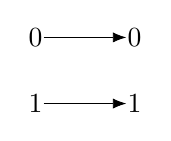
\begin{tikzpicture}[x=0.42cm,y=0.42cm,baseline=-0.5ex]
  \node[chnode] (x0) at (0, 1) {$0$};
  \node[chnode] (x1) at (0,-1) {$1$};
  \node[chnode] (y0) at (3, 1) {$0$};
  \node[chnode] (y1) at (3,-1) {$1$};
  \draw[charr] (x0)--(y0);
  \draw[charr] (x1)--(y1);
\end{tikzpicture}%
}{\(Y=X\), \(H(Y|X)=0\).\\
\(I(X;Y)=H(Y)=H(X)\le1\).\\
均匀输入达到 \(C=1\).}

\chcard{BSC\((p)\)}{%
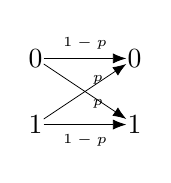
\begin{tikzpicture}[x=0.42cm,y=0.42cm,baseline=-0.5ex]
  \node[chnode] (x0) at (0, 1) {$0$};
  \node[chnode] (x1) at (0,-1) {$1$};
  \node[chnode] (y0) at (3, 1) {$0$};
  \node[chnode] (y1) at (3,-1) {$1$};
  \draw[charr] (x0)--node[above,font=\tinytight] {$1-p$}(y0);
  \draw[charr] (x1)--node[below,font=\tinytight] {$1-p$}(y1);
  \draw[charr] (x0)--node[above right=-1pt,font=\tinytight] {$p$}(y1);
  \draw[charr] (x1)--node[below right=-1pt,font=\tinytight] {$p$}(y0);
\end{tikzpicture}%
}{\(Y=X\oplus Z,\ Z\sim\mathrm{Bern}(p)\).\\
\(H(Y|X)=H(p)\), \(H(Y)\le1\).\\
均匀输入使 \(Y\) 均匀，\(C=1-H(p)\).}

\topic{Replace These Blocks}
后续按考试检索顺序填：定义 \(\to\) 恒等式 \(\to\) 不等式 \(\to\) 定理 \(\to\) 算法 \(\to\) 例题模式 \(\to\) 易错点。

\note{Fitting ladder}{若出第 3 页：先删重复散文，合并相邻主题，缩图 \(5\%-15\%\)，再调行距；最后才降字号。若不足两页：补高频定理、证明骨架、等号条件和小图。}

% ----------------------------------------------------------------------
% Paste compressed course content below.
% Keep comments out of the final PDF; they do not render.
% Use \newpage only if you intentionally want to force page 2.
% ----------------------------------------------------------------------

\chap{Page 1 Content}
\topic{Topic A}
\fact{Formula}{\(a=b+c,\quad b=\sum_i p_i x_i\)}
\fact{Use when}{看到关键词/条件时怎么套。}
\fact{Trap}{不要把条件 A 和条件 B 混用。}

\topic{Topic B}
\twoline{f(x)=\arg\max_{\theta} L(\theta;x)}
{g(x)=\min_q \max_p R(p,q)}
短句解释即可。把长证明压成关键一步。

\newpage

\chap{Page 2 Content}
\topic{Topic C}
\fact{Theorem}{条件：写清独立性、极限、分布或矩阵结构。结论：写可直接代入的式子。}
\note{Converse}{令消息 \(W\)，从 \(H(W)\) 出发，用 Fano / data processing / single-letterization 推上界。}
\note{Achievability}{随机构造 \(\to\) 典型性/覆盖/打包 \(\to\) union bound \(\to\) 误差趋零。}

\topic{Checklist}
\begin{itemize}
  \item 页数：必须 exactly \(2\) pages；
  \item 公式：用 LaTeX 真公式，不要渲染成图片；
  \item 图片：只保留能省字或帮助判断结构的图；
  \item 文字：每句服务于考试检索。
\end{itemize}

\end{multicols*}
\end{document}
